\documentclass[tikz,border=4pt]{standalone}
\usepackage{amsmath}
\usepackage[T1]{fontenc}
\usetikzlibrary{arrows.meta,calc}

\definecolor{KetteringBlue}{HTML}{1E4B99}
\definecolor{rodBlue}{HTML}{2E7CD6}
\definecolor{aNcol}{HTML}{1E7B1E}      % dark green for normal component
\definecolor{aTcol}{HTML}{C13030}      % dark red for tangential component
\definecolor{aBcol}{HTML}{1E4B99}      % dark blue for resultant a_B

\begin{document}
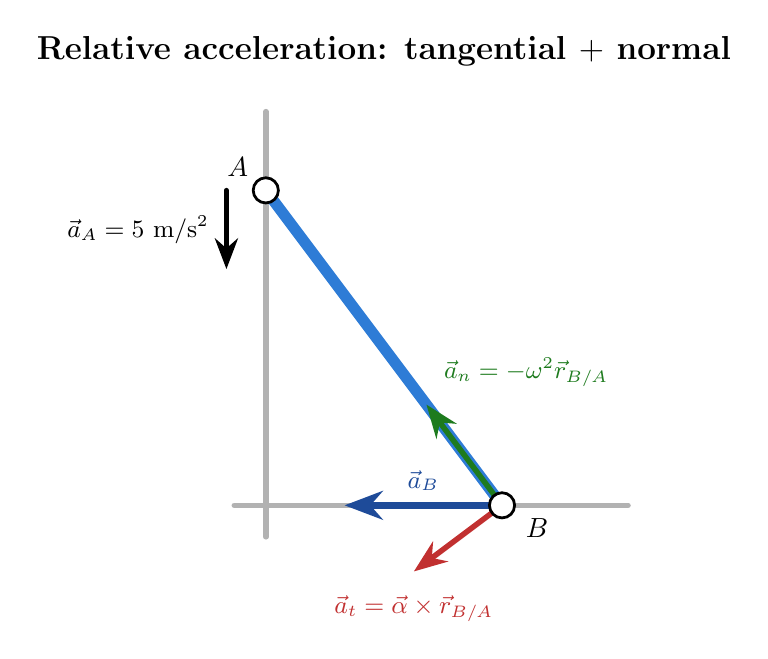
\begin{tikzpicture}[
  >=Stealth,
  line cap=round,
  every node/.style={font=\small}
]
  \coordinate (A) at (0,4);
  \coordinate (B) at (3,0);

  % Wall and floor
  \draw[gray!60, line width=2.0pt] (-0.4,0) -- (4.6,0);
  \draw[gray!60, line width=2.0pt] (0,-0.4) -- (0,5.0);

  % Rod
  \draw[rodBlue, line width=4pt] (A) -- (B);

  % a_A arrow at A (downward, drawn outside wall to the left)
  \draw[->, line width=1.8pt, black] (-0.5,4) -- (-0.5,3.0);
  \node[anchor=east] at (-0.6,3.5) {$\vec a_A = 5\ \mathrm{m/s^2}$};

  % a_n vector: from B toward A, length 1.6 along rod direction (-3/5, 4/5)
  \coordinate (anEnd) at ($(B)+(-0.96,1.28)$);
  \draw[->, line width=2.0pt, aNcol] (B) -- (anEnd);
  \node[anchor=south west, aNcol] at ($(anEnd)+(0.1,0.1)$)
    {$\vec a_n = -\omega^2 \vec r_{B/A}$};

  % a_t vector: perpendicular to rod, down-left direction (-4/5, -3/5), length 1.4
  \coordinate (atEnd) at ($(B)+(-1.12,-0.84)$);
  \draw[->, line width=2.0pt, aTcol] (B) -- (atEnd);
  \node[anchor=north, aTcol] at ($(atEnd)+(0,-0.18)$)
    {$\vec a_t = \vec\alpha \times \vec r_{B/A}$};

  % a_B vector: horizontal left from B (starts AT B, drawn on top of floor)
  \coordinate (aBEnd) at ($(B)+(-2.0,0)$);
  \draw[->, line width=2.4pt, aBcol] (B) -- (aBEnd);
  \node[anchor=south, aBcol] at ($(B)!0.5!(aBEnd)+(0,0.06)$) {$\vec a_B$};

  % Slider markers at A and B
  \fill[white] (A) circle (0.16);
  \draw[black, line width=1pt] (A) circle (0.16);
  \fill[white] (B) circle (0.16);
  \draw[black, line width=1pt] (B) circle (0.16);

  % Point labels
  \node[font=\bfseries, anchor=south east] at ($(A)+(-0.1,0.05)$) {$A$};
  \node[font=\bfseries, anchor=north west] at ($(B)+(0.18,-0.05)$) {$B$};

  % Title
  \node[font=\bfseries\large, anchor=south] at (1.5,5.45)
    {Relative acceleration: tangential $+$ normal};
\end{tikzpicture}
\end{document}
